
\section{Séance 3}

\vspace*{1cm}

\begin{exo}
Construisez un code de Gray d'ordre $5$ sur base du code de Gray d'ordre $4$ ci-dessous.\\
0000,0100,1100,1000,1010,1110,0110,0010,0011,0111,1111,1011,1001,1101,0101,0001
\end{exo}

Pour consuire le code de Gray d'ordre $n+1$ à partir du code de Gray d'ordre $n$, il suffit de rajouter un 0 à chaque élément, dans l'ordre, puis repartir dans le sens inverse en rajoutant des 1.

Donc, le code de Gray d'ordre 5 est: 

0000\textcolor{red}{0}, 0100\textcolor{red}{0}, 1100\textcolor{red}{0}, 1000\textcolor{red}{0}, 1010\textcolor{red}{0}, 1110\textcolor{red}{0}, 0110\textcolor{red}{0}, 0010\textcolor{red}{0}, 0011\textcolor{red}{0}, 0111\textcolor{red}{0}, 1111\textcolor{red}{0}, 1011\textcolor{red}{0}, 1001\textcolor{red}{0}, 1101\textcolor{red}{0}, 0101\textcolor{red}{0}, 0001\textcolor{red}{0}, 

0001\textcolor{red}{1}, 0101\textcolor{red}{1}, 1101\textcolor{red}{1}, 1001\textcolor{red}{1}, 1011\textcolor{red}{1}, 1111\textcolor{red}{1}, 0111\textcolor{red}{1}, 0011\textcolor{red}{1}, 0010\textcolor{red}{1}, 0110\textcolor{red}{1}, 1110\textcolor{red}{1}, 1010\textcolor{red}{1}, 1000\textcolor{red}{1}, 1100\textcolor{red}{1}, 0100\textcolor{red}{1}, 0000\textcolor{red}{1}
%-----------------------------------------------------------------

\begin{exo}
Dans le graphe ci-dessous, on donne un couplage de cardinal maximal. En utilisant la preuve du th\'eor\`eme de K\"onig vue au cours, trouvez un transversal de cardinal minimal.
\end{exo}

\begin{figure}[!h]
\begin{center}
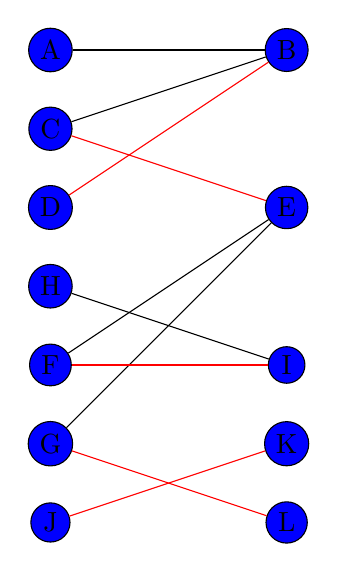
\begin{tikzpicture}

\tikzstyle{every node}=[draw,circle,fill=black,minimum size=10pt,inner sep=2pt]
\tikzstyle{every label}=[position=above]

\node[circle,fill=blue] (v7) at (0,0) {D};
\node[circle,fill=blue] (v8) at (0,-1) {H};
\node[circle,fill=blue] (v10) at (0,-2) {F};
\node[circle,fill=blue] (v12) at (0,-3) {G};
\node[circle,fill=blue] (v5) at (0,1) {C};
\node[circle,fill=blue] (v1) at (0,2) {A};
\node[circle,fill=blue] (v3) at (3,2) {B};
\node[circle,fill=blue] (v4) at (3,0) {E};
\node[circle,fill=blue] (v9) at (3,-2) {I};
\node[circle,fill=blue] (v11) at (3,-3) {K};
\node[circle,fill=blue] (v6) at (3,-4) {L};
\node[circle,fill=blue] (v13) at (0,-4) {J};
\draw  (v1) -- (v3);
\draw  (v5) -- (v3);
\draw  (v8) -- (v9);
\draw  (v10) -- (v4);
\draw  (v12) -- (v4);

\draw[red] (v7) -- (v3);
\draw[red] (v5) -- (v4);
\draw[red] (v10) -- (v9);
\draw[red] (v12) -- (v6);
\draw[red] (v11) -- (v13);
\end{tikzpicture}
\end{center}
\caption{}
\end{figure}

<TO DO>

%-----------------------------------------------------------------

\begin{exo}
Sur $\R^2$, on d\'efinit les relations suivantes:
\[(x,y)\mathcal{R}(x',y') \Leftrightarrow x \leq x' \mathrm{~et~} y \leq y', \]
\[(x,y)\mathcal{S}(x',y') \Leftrightarrow (x < x') \mathrm{~ou~} (x = x' \mathrm{~et~} y \leq y').\]
Est-ce que les relations $\mathcal{R}$ et $\mathcal{S}$ sont des ordres?
\end{exo}

<TO DO>

%-----------------------------------------------------------------

\begin{exo}
Consid\'erons le graphe biparti (bipartition donn\'ee par une coloration des sommets) ci-dessous. Sur l'ensemble de ses sommets, on d\'efinit la relation $u\leq v$ pour $u,v$ des sommets tels que $u$ est un sommet rouge et $\{u,v\}$ est une ar\^ete. On pose aussi $u\leq u$ pour tout sommet $u$. \\
\begin{enumerate}[(a)]
\item V\'erifiez que $\leq$ est un ordre partiel.
\item Construisez une partition des sommets par $k$ cha\^ines et trouvez une anticha\^ine contenant $k$ \'el\'ements.
\item D\'eduisez-en un couplage de cardinalit\'e maximale et un transversal de cardinalit\'e minimale. 
\item (Bonus) Sur base de ce qui est fait ci-dessus, prouvez que le th\'eor\`eme de K\"onig implique le th\'eor\`eme de Dilworth.
\end{enumerate}
\end{exo}

\begin{figure}[!h]
\begin{center}
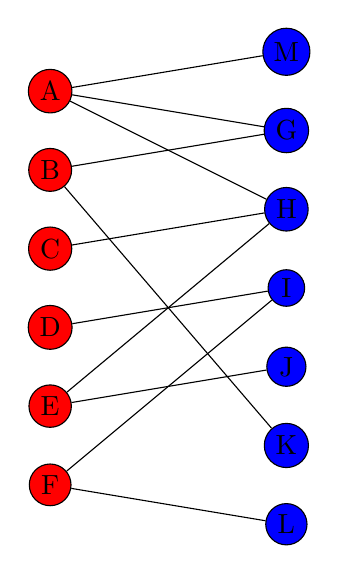
\begin{tikzpicture}

\tikzstyle{every node}=[draw,circle,fill=black,minimum size=10pt,inner sep=2pt]
\tikzstyle{every label}=[position=above]

\node[circle,fill=red] (v7) at (0,0) {C};
\node[circle,fill=red] (v8) at (0,-1) {D};
\node[circle,fill=red] (v10) at (0,-2) {E};
\node[circle,fill=red] (v12) at (0,-3) {F};
\node[circle,fill=red] (v5) at (0,1) {B};
\node[circle,fill=red] (v1) at (0,2) {A};
\node[circle,fill=blue] (v3) at (3,1.5) {G};
\node[circle,fill=blue] (v2) at (3,2.5) {M};
\node[circle,fill=blue] (v4) at (3,0.5) {H};
\node[circle,fill=blue] (v9) at (3,-0.5) {I};
\node[circle,fill=blue] (v11) at (3,-1.5) {J};
\node[circle,fill=blue] (v6) at (3,-2.5) {K};
\node[circle,fill=blue] (v13) at (3,-3.5) {L};
\draw  (v1) edge (v2);
\draw  (v1) edge (v3);
\draw  (v1) edge (v4);
\draw  (v5) edge (v3);
\draw  (v5) edge (v6);
\draw  (v7) edge (v4);
\draw  (v8) edge (v9);
\draw  (v10) edge (v4);
\draw  (v10) edge (v11);
\draw  (v12) edge (v9);
\draw  (v12) edge (v13);
\end{tikzpicture}
\end{center}
\caption{}
\end{figure}

%-----------------------------------------------------------------